% 等离子体物理基础第三次作业

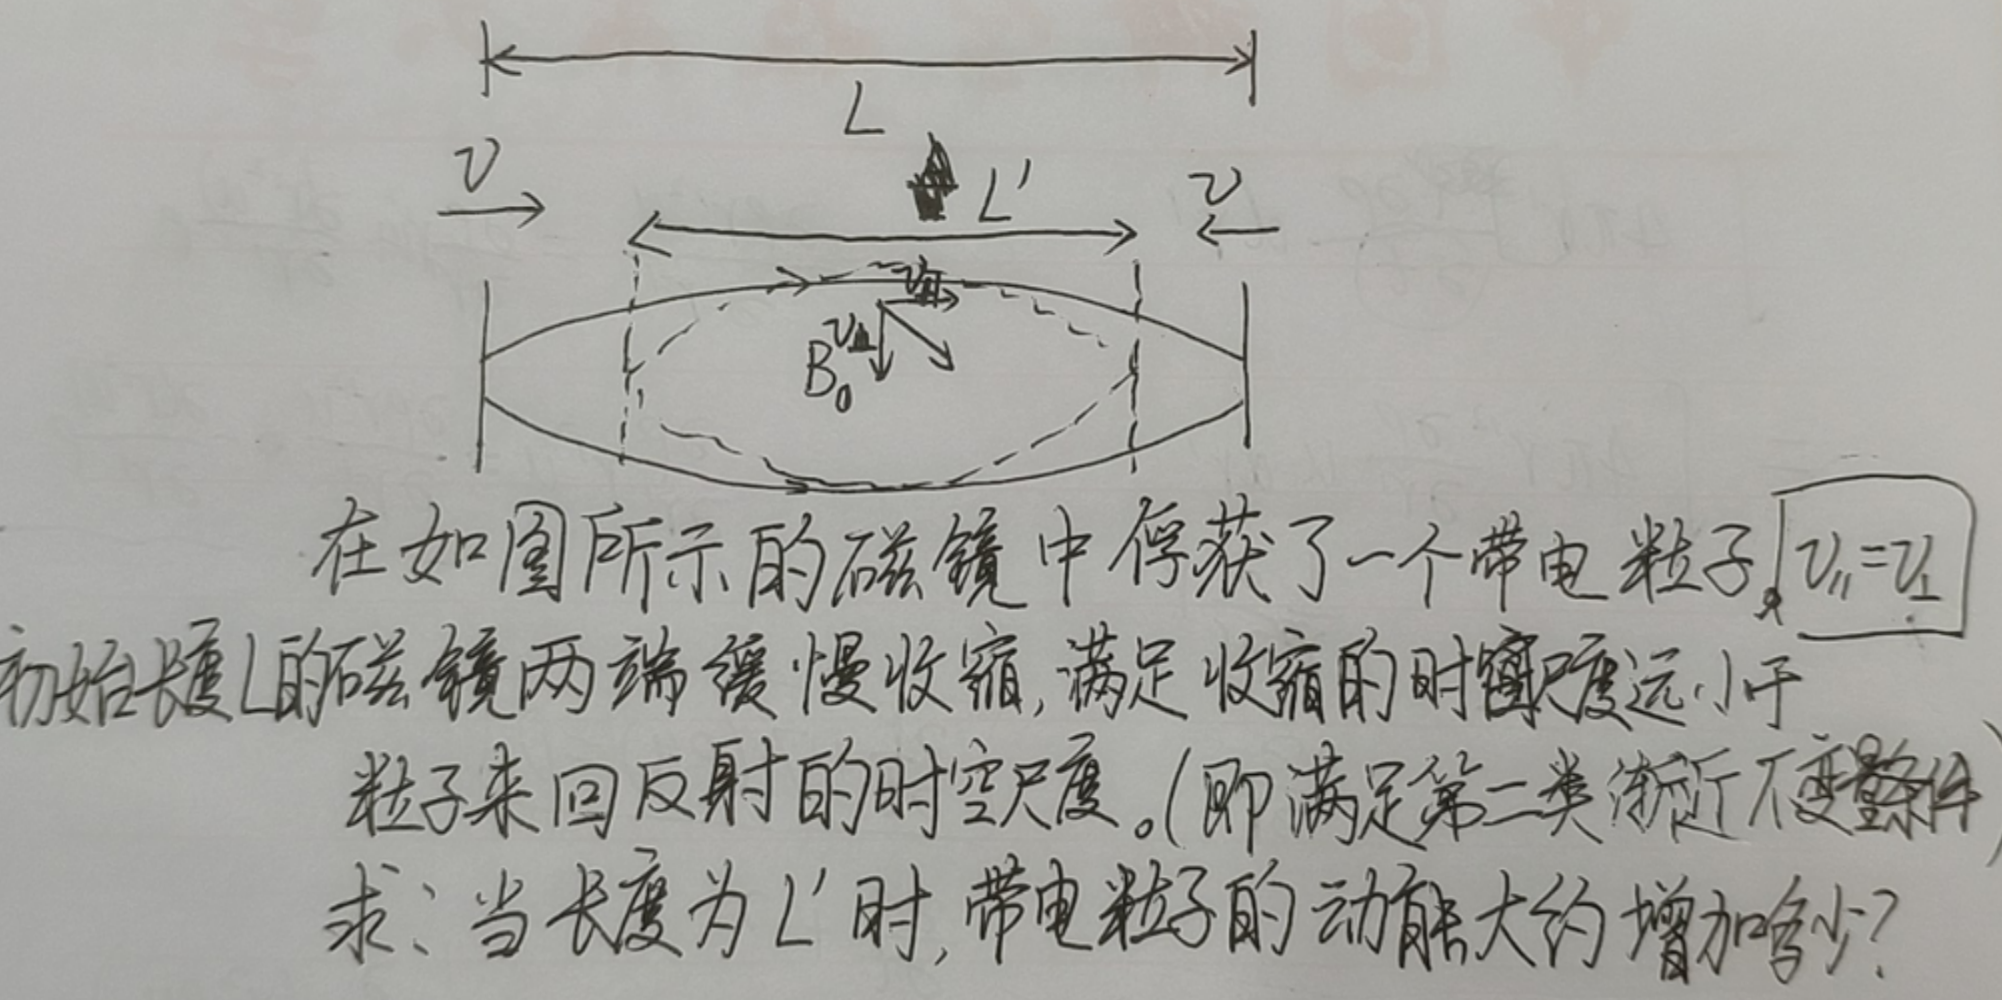
\includegraphics[width=\textwidth]{figures/2022-10-21T120911+0800.png}
\section{磁镜缓变作业的解}
倘若这是一个普遍情况,那么我设一个特殊情况必然得到相同的结论。
不妨设对称轴上的磁场表达式为
\begin{equation}
B_z = B_0 (1 + \alpha^2 z^2)
\label{eq:B}
\end{equation}
,其中\(\alpha>0, B_0\)都为常数。
初始条件,在\(z=0\)处,\(B_z = B_0\),\( v_\perp = v_\parallel\),
在一个较短的时间内,满足能量守恒,不妨设初始的总速度为
\begin{equation}
  v^2 = v_\parallel^2 + v_\perp^2 = 2 v_\perp^2.
\end{equation}
同样,在一个较短的时间内,设\(z=\frac{L}{2}\)处的磁场为\(B_1\),由于磁矩守恒
\begin{equation}
  \mu = \frac{1}{2} m v_\perp^2 \big/ B_0 =
\frac{1}{2} m v^2 \big/ B_1 
\end{equation}
可得
\begin{equation}
  B_1 = 2 B_0
\end{equation}
代入\cref{eq:B}可得
\begin{equation}
  \frac{1}{\alpha} = \frac{L}{2}.
  \label{eq:L}
\end{equation}
\begin{equation}
 \because \mu = \frac{m v_\perp^2}{2 B_z} \implies \mu B_0 ( 1 + \alpha^2 z^2 ) = \frac{1}{2} m v_\perp^2
\end{equation}
\begin{equation}
  \therefore v_\parallel = v^2 - v_\perp^2 = \frac{\mu_0 B}{m} - \frac{2 \mu_0 B}{m} \alpha^2 z^2
\end{equation}
\begin{equation}
  \dv{z}{t} = \sqrt{\frac{\mu_0 B_0}{m}} \sqrt{1 - 2 \alpha^2 z^2}
\end{equation}
\begin{equation}
   \implies z = \frac{\sqrt{2}}{2 \alpha} \sin(\sqrt{\frac{2 \mu_0 B_0}{m}}\alpha t + \phi)
\end{equation}
显然,是简谐运动。
设\(\theta = \sqrt{\frac{2 \mu_0 B_0}{m}}\alpha t + \phi\) 则有 \(z = \sqrt{2} / (2 \alpha) \sin \theta\),
由于
\begin{equation}
  J = \int_a^b v_\parallel \dd{z}
\end{equation}
其中,\(\alpha  = - \sqrt{2} / ( 2 \alpha ), b = \sqrt{2} / ( 2 \alpha )\),
因此
\begin{equation*}
  \theta_a = - \frac{\pi}{2}, 
  \theta_b = \frac{\pi}{2} 
\end{equation*}
\begin{equation}
  J = \int_a^b v_\parallel \dd{z} = \int v_\parallel  v_\parallel \dd{t} = \frac{1}{\alpha} \sqrt{ \frac{m}{2 \mu B_0} } \int_{\theta_a}^{\theta_b} v_\parallel^2 \dd{\theta}
\end{equation}
其中
\begin{equation}
  \dd{t} = \frac{1}{\alpha} \sqrt{\frac{m}{2\mu B_0}} \dd{\theta}, v_\parallel^2 = \left(\dv{z}{t}\right)^2
\end{equation}
\begin{equation}
  \begin{aligned}
    \therefore J &= \frac{1}{\alpha} \sqrt{\frac{m}{2 \mu B_0}} \int_{- \frac{\pi}{2}}^{\frac{\pi}{2}} \frac{\mu B_0}{m} \sin[2](\theta) \dd{\theta} \\
                 &= \frac{\pi}{2 \alpha} \sqrt{\frac{\mu B_0}{2 m}} = {\rm constant} \\
                 &= \frac{\pi}{2 \alpha} \sqrt{\frac{(1/2) m v_\perp^2}{2 m}}  \quad \text{代入\(z=0\)时的磁矩表达式} \\
                 &= \frac{\pi}{2 \alpha} \sqrt{\frac{(1/4) m v^2}{2 m}} =\frac{\pi}{2 \alpha} \sqrt{\frac{(1/2) E_k}{2 m}} 
  \end{aligned}
\end{equation}
设初态动能为\(E_k\),末态动能为\(E_k'\)
\begin{equation}
  \therefore J = 
\frac{\pi}{2 \alpha} \sqrt{\frac{(1/2) E_k}{2 m}} =
\frac{\pi}{2 \alpha'} \sqrt{\frac{(1/2) E_k'}{2 m}} 
\end{equation}
\begin{equation}
  \therefore 
  \left(\frac{1}{\alpha}\right)^2 E_k = 
  \left(\frac{1}{\alpha'}\right)^2 E_k'
\end{equation}
把\cref{eq:L}代入上式,可得
\begin{equation}
  \therefore 
  L^2 E_k = 
  L'^2 E_k'
\end{equation}
\begin{equation}
  \begin{aligned}
    \therefore \Delta E_k = E_k' - E_k &= \left(\left(\frac{L}{L'}\right)^2-1\right) E_k \\
                                   &= \left(\left(\frac{L}{L'}\right)^2-1\right) \cdot (1 / 2) mv^2\\
                                   &= \left(\left(\frac{L}{L'}\right)^2-1\right) \cdot mv_\perp^2
  \end{aligned}
\end{equation}




%%% vim: set ts=2 sts=2 sw=2 isk+=\: et cc=+1 formatoptions+=mM:
